%%%%%%%%%%%%%%%%%%%%%%%%%%%%%%%%%%%%%%%%%%%%%%%%%%%%%%%%%%%%%%%%%%%%%%%%%%%%%%%%
%% Plantilla de memoria en LaTeX para la EIF - Universidad Rey Juan Carlos
%%
%% Por Gregorio Robles <grex arroba gsyc.urjc.es>
%%     Grupo de Sistemas y Comunicaciones
%%     Escuela de Ingeniería de Fuenlabrada
%%     Universidad Rey Juan Carlos
%% (muchas ideas tomadas de Internet, colegas del GSyC, antiguos alumnos...
%%  etc. Muchas gracias a todos)
%%
%% La última versión de esta plantilla está siempre disponible en:
%%     https://github.com/gregoriorobles/plantilla-memoria
%%
%% Para obtener PDF, ejecuta en la shell:
%%   make
%% (las imágenes deben ir en PNG o JPG)

%%%%%%%%%%%%%%%%%%%%%%%%%%%%%%%%%%%%%%%%%%%%%%%%%%%%%%%%%%%%%%%%%%%%%%%%%%%%%%%%

\documentclass[a4paper, 12pt]{book}
%\usepackage[T1]{fontenc}

\usepackage[a4paper, left=2.5cm, right=2.5cm, top=3cm, bottom=3cm]{geometry}
\usepackage{times}
\usepackage[utf8]{inputenc}
\usepackage[spanish]{babel} % Comenta esta línea si tu memoria es en inglés
\usepackage{url}
%\usepackage[dvipdfm]{graphicx}
\usepackage{graphicx}
\usepackage{float}  %% H para posicionar figuras
\usepackage[nottoc, notlot, notlof, notindex]{tocbibind} %% Opciones de índice
\usepackage{latexsym}  %% Logo LaTeX

\title{Memoria del Proyecto}
\author{Nombre del autor}

\renewcommand{\baselinestretch}{1.5}  %% Interlineado

\begin{document}


%%%%%%%%%%%%%%%%%%%%%%%%%%%%%%%%%%%%%%%%%%%%%%%%%%%%%%%%%%%%%%%%%%%%%%%%%%%%%%%%
% PORTADA

\begin{titlepage}
\begin{center}
\includegraphics[scale=0.6]{img/URJ_logo_Color_POS.png}

\vspace{1.75cm}

\LARGE
ESCUELA DE INGENIERÍA DE FUENLABRADA
\vspace{1cm}

\LARGE
INGENIERÍA EN SISTEMAS AUDIOVISUALES Y MULTIMEDIA

\vspace{1cm}
\LARGE
\textbf{TRABAJO FIN DE GRADO/MÁSTER}

\vspace{2cm}

\Large
AUTOMATIZACIÓN DE TAREAS CON POWERSHELL

\vspace{2cm}

\large
Autora : Patricia Castaño Sánchez \\
Tutor : Dr. Gregorio Robles \\
\vspace{1cm}

\large
Curso académico 2022/2023

\end{center}
\end{titlepage}

\newpage
\mbox{}
\thispagestyle{empty} % para que no se numere esta pagina



%%%%%%%%%%%%%%%%%%%%%%%%%%%%%%%%%%%%%%%%%%%%%%%%%%%%%%%%%%%%%%%%%%%%%%%%%%%%%%%%
%%%% Para firmar
\clearpage
\pagenumbering{gobble}
\chapter*{}

\vspace{-4cm}
\begin{center}
\LARGE
\textbf{Trabajo Fin de Grado/Máster}

\vspace{1cm}
\large
Automatización de Tareas con Powershell

\vspace{1cm}
\large
\textbf{Autora :} Patricia Castaño Sánchez \\
\textbf{Tutor :} Dr. Gregorio Robles

\end{center}

\vspace{1cm}
La defensa del presente Proyecto Fin de Carrera se realizó el día \qquad$\;\,$ de \qquad\qquad\qquad\qquad \newline de 2023, siendo calificada por el siguiente tribunal:


\vspace{0.5cm}
\textbf{Presidente:}

\vspace{1.2cm}
\textbf{Secretario:}

\vspace{1.2cm}
\textbf{Vocal:}


\vspace{1.2cm}
y habiendo obtenido la siguiente calificación:

\vspace{1cm}
\textbf{Calificación:}


\vspace{1cm}
\begin{flushright}
Fuenlabrada, a \qquad$\;\,$ de \qquad\qquad\qquad\qquad de 2023
\end{flushright}

%%%%%%%%%%%%%%%%%%%%%%%%%%%%%%%%%%%%%%%%%%%%%%%%%%%%%%%%%%%%%%%%%%%%%%%%%%%%%%%%
%%%% Dedicatoria

\chapter*{}
\pagenumbering{Roman} % para comenzar la numeracion de paginas en numeros romanos
\begin{flushright}
\textit{Dedicado a \\
mi familia}
\end{flushright}

%%%%%%%%%%%%%%%%%%%%%%%%%%%%%%%%%%%%%%%%%%%%%%%%%%%%%%%%%%%%%%%%%%%%%%%%%%%%%%%%
%%%% Agradecimientos

\chapter*{Agradecimientos}
%\addcontentsline{toc}{chapter}{Agradecimientos} % si queremos que aparezca en el índice
\markboth{AGRADECIMIENTOS}{AGRADECIMIENTOS} % encabezado 

A mis padres, hermano, y familia por su eterno apoyo y cariño.

%%%%%%%%%%%%%%%%%%%%%%%%%%%%%%%%%%%%%%%%%%%%%%%%%%%%%%%%%%%%%%%%%%%%%%%%%%%%%%%%
%%%% Resumen

\chapter*{Resumen}
%\addcontentsline{toc}{chapter}{Resumen} % si queremos que aparezca en el índice
\markboth{RESUMEN}{RESUMEN} % encabezado

Powershell es un lenguaje de scripting desarrollado por Microsoft, que se utiliza principalmente para automatizar tareas en sistemas operativos Windows y en otros productos de Microsoft.
\\

Powershell utiliza una sintaxis similar a la de los comandos de línea de comandos (CMD), pero ofrece una amplia gama de funciones y características avanzadas, como la capacidad de trabajar con objetos en lugar de solo texto y la posibilidad de ejecutar comandos remotos en otros equipos.
\\

En resumen, Powershell es un lenguaje de programación de scripts que permite a los administradores de sistemas automatizar tareas y realizar una amplia variedad de tareas en sistemas operativos Windows y otros productos de Microsoft de manera eficiente y sencilla.
\\

Este proyecto trata de mostrar el uso de dicho lenguaje aplicado en casos reales de empresa para la automatización de tareas. Las tecnologías que se verán involucradas en este trabajo, junto a este lenguaje, serán Active Directory, SQL, Sharepoint y System Center Configuration Manager.
\\

En este trabajo se enseñarán ejemplos de tareas existentes y en uso en la empresa a día de hoy para mostrar la eficacia del lenguaje Powershell a la hora de automatizar y simplificar tareas manuales por parte de los trabajadores.
\\

Hay que tener en cuenta que, aunque en este trabajo se presenten ejemplos con las tecnologías anteriormente citadas, Powershell es capaz de trabajar con cualquier tecnología de Microsoft como Hyper-V, Virtual Machine Manager, etc. También es posible modificar características de los equipos como el registro Windows, activar/desactivar servicios, cambiar nombre de red, etc.


%%%%%%%%%%%%%%%%%%%%%%%%%%%%%%%%%%%%%%%%%%%%%%%%%%%%%%%%%%%%%%%%%%%%%%%%%%%%%%%%
%%%%%%%%%%%%%%%%%%%%%%%%%%%%%%%%%%%%%%%%%%%%%%%%%%%%%%%%%%%%%%%%%%%%%%%%%%%%%%%%
% ÍNDICES %
%%%%%%%%%%%%%%%%%%%%%%%%%%%%%%%%%%%%%%%%%%%%%%%%%%%%%%%%%%%%%%%%%%%%%%%%%%%%%%%%

% Las buenas noticias es que los índices se generan automáticamente.
% Lo único que tienes que hacer es elegir cuáles quieren que se generen,
% y comentar/descomentar esa instrucción de LaTeX.

%%%% Índice de contenidos
\tableofcontents 
%%%% Índice de figuras
\cleardoublepage
%\addcontentsline{toc}{chapter}{Lista de figuras} % para que aparezca en el indice de contenidos
\listoffigures % indice de figuras
%%%% Índice de tablas
%\cleardoublepage
%\addcontentsline{toc}{chapter}{Lista de tablas} % para que aparezca en el indice de contenidos
%\listoftables % indice de tablas


%%%%%%%%%%%%%%%%%%%%%%%%%%%%%%%%%%%%%%%%%%%%%%%%%%%%%%%%%%%%%%%%%%%%%%%%%%%%%%%%
%%%%%%%%%%%%%%%%%%%%%%%%%%%%%%%%%%%%%%%%%%%%%%%%%%%%%%%%%%%%%%%%%%%%%%%%%%%%%%%%
% INTRODUCCIÓN %
%%%%%%%%%%%%%%%%%%%%%%%%%%%%%%%%%%%%%%%%%%%%%%%%%%%%%%%%%%%%%%%%%%%%%%%%%%%%%%%%

\cleardoublepage
\chapter{Introducción}
\label{sec:intro} % etiqueta para poder referenciar luego en el texto con ~\ref{sec:intro}
\pagenumbering{arabic} % para empezar la numeración de página con números

Este trabajo surge para mostrar la necesidad de las empresas de simplificar y agilizar tareas rutinarias y repetitivas de sus empleados para poder aprovechar el tiempo de estos de una manera mucho más eficiente sin tener que perderlo en tareas manuales que pueden automatizarse, consiguiendo además un mejor control de dichas tareas evitando errores humanos.
\\

Este trabajo fin de grado tratará de demostrar cómo, uniendo las tecnologías SQL, Active Directory, Sharepoint, System Center Configuration Manager y Powershell, se automatiza la actualización de datos de los trabajadores almacenados en el directorio activo.
\\

Se pondrá el foco en tres tareas reales para explicar de manera específica la utilidad de automatizar tareas en la empresa, y se añadiran, como muestra de que hay muchas más tareas tratadas, otros ejemplos reales y en uso de trabajos automatizados en la empresa. Hay que tener en cuenta que, por norma general, cualquier labor repetitiva llevada a cabo por los técnicos, se puede llegar a automatizar, algunos ejemplos en uso en la empresa son:

\begin{itemize}
\item Creación de usuarios en Active Directory

\item Cambio de contraseña caducada

\item Actualizar listas de Sharepoint con usuarios dados de alta en el directorio activo

\item Chequear número de licencias de correo

\item Chequear fecha de caducidad de certificado personal

\item Copiar elementos de una lista entre dos listas de Sharepoint

\item Eliminar elementos de una lista de Sharepoint

\item Crear una colección de equipos en System Center Configuration Manager (SCCM)

\item Chequear fecha de caducidad de contraseña personal
\end{itemize}


\section{Contexto}
\label{sec:contexto}

En esta sección se describe el contexto en el que se encuentran los tres scripts de muestra para este trabajo de fin de grado.

\subsection{Actualización de información de usuarios}
\label{subsec:Actualización de información de usuarios}

En el primer ejemplo de caso real utilizado para desarrollar en este trabajo fin de grado, la empresa cuenta con una base de datos Oracle que recoge la información de los trabajadores gestionada por el equipo de Recursos Humanos. Los trabajadores, en una de sus muchas tareas, acceden de forma manual a dicha base de datos y, uno por uno, van comparando la información de cada usuario almacenada con la información de la que disponen en el directorio activo. Esto puede suponer varias horas de trabajo.
\\

Para reducir el tiempo del trabajador en esta tarea, se estudia automatizarla con lenguaje Powershell.
\\

Dicha base de datos se almacena en un servidor al que se accederá a través de lenguaje Powershell para recuperar la información deseada de cada empleado y replicarla en objetos de Active Directory, los cuales son necesarios para tener un control de los trabajadores dados de alta en la empresa, así como su información personal, servicios de la empresa a los que puede acceder cada uno de ellos, licencias dadas de alta, etc.

\subsection{Creación de colección de equipos en SCCM}
\label{Creación de colección de equipos en SCCM}

La empresa trabaja con la tecnología de System Center Configuration Manager (SCCM), que se encarga, entre otras cosas, de administrar las actualizaciones de los equipos de los empleados.
\\

Estas actualizaciones de equipo las prueban los técnicos del departamento de Desktop y de Sistemas antes de desplegarse al resto de usuarios de la empresa. Dichas actualizaciones se configuran con una determinada fecha de despliegue y de instalación, por lo que la empresa crea dos grupos con los equipos de los técnicos que van a probarlas por si, en caso de que la actualización afectase al funcionamiento del equipo, no se vieran todos los técnicos afectados.
\\

Los objetos del Active Directory correspondientes a los usuarios del departamento de Desktop y de Sistemas se encuentran en un grupo de éste directorio activo el cual es dinámico ya que se va actualizando con los nuevos integrantes del departamento o las bajas de éste.
\\

Se decide crear un script para automatizar esta tarea y evitar tener que ocupar un técnico en revisar dicho grupo de Active Directory y crear las colecciones de los equipos correspondientes en SCCM de forma manual, lo que conllevaría buscar usuario por usuario en la herramienta de SCCM y asignar su equipo a una de estas dos colecciones.
\\

Este script consultará el grupo del directorio activo, buscará en SCCM el equipo asignado a cada usuario de este grupo y los repartirá de forma aleatoria en dos colecciones de actualizaciones en SCCM.

\subsection{Actualización de lista Sharepoint con usuarios con soporte}
\label{Actualización de lista Sharepoint con usuarios con soporte}

La empresa da soporte a mas de 5000 empleados de otras iniciativas y dispone de diferentes tipos de soporte y servicios que van desde únicamente soporte de equipo físico hasta soporte de licencia de correo electrónico, soporte de Microsoft Outlook, etc.
\\

Los técnicos del departamento de Desktop necesitan tener una lista que contenga todos los usuarios a los que se les da soporte y qué tipo de soporte se les da para saber, en caso de incidencia, qué servicios se ofrece a cada usuario.
\\

Estos tipos de soporte se deciden dependiendo de una serie de parámetros que deben cumplir los usuarios como son: tipo de empleado (propio, colaborador o becario), iniciativa para la que trabaja, plan de licencia,…
\\

Esta tarea sería muy complicada hacerla de forma manual ya que existen más de 5000 empleados a los que se les da soporte y la lista de parámetros es larga, por lo que se decide crear un script que rellene una lista en Sharepoint con la información requerida por los técnicos de la empresa para saber cómo tienen que actuar en caso de incidencia con cada usuario.
\\

Este script consulta tanto la base de datos Oracle, que contiene la información de todos los usuarios, como los usuarios en Active Directory, dando preferencia a la base de datos en caso de encontrar el mismo usuario en ambos lados; chequea la información de estos usuarios contra una lista de Sharepoint en la que se han establecido unos parámetros para cada tipo de soporte y, dependiendo los parámetros que cumpla cada usuario, se añaden a otra lista Sharepoint en la que se indica tanto la información del usuario (nombre, apellidos, dirección de correo electrónico, iniciativa para la que trabaja, matrícula, etc.) como el tipo de soporte que tiene y los servicios contratados.


\section{Estructura de la memoria}
\label{sec:estructura}

La estructura de este trabajo se divide seis capítulos, tales que:

\begin{itemize}
\item Capítulo 1. Introducción.
Se explica cómo surge la necesidad de este trabajo, para qué se usa y el contexto en el que se desarrolla.

\item Capítulo 2. Objetivos.
Se explica el objetivo general del trabajo y los objetivos específicos de la automatización de una de las grandes tareas llevadas a cabo por la empresa.

\item Capítulo 3. Estado del arte.
Se explica cada una de las tecnologías involucradas en el trabajo.

\item Capítulo 4. Diseño e Implementación.
Se explica en qué consiste el trabajo aplicado en la empresa y se muestran casos reales de tareas que están en funcionamiento.

\item Capítulo 5. Experimentos, validación y resultados.
Se muestran varios ejemplos de experimentos con diferentes tareas reales de la empresa, mostrando el resultado en imágenes.

\item Capítulo 6. Conclusiones.
Se explican las conclusiones que se adquieren con este trabajo y las lecciones aprendidas.

\end{itemize}





%%%%%%%%%%%%%%%%%%%%%%%%%%%%%%%%%%%%%%%%%%%%%%%%%%%%%%%%%%%%%%%%%%%%%%%%%%%%%%%%
%%%%%%%%%%%%%%%%%%%%%%%%%%%%%%%%%%%%%%%%%%%%%%%%%%%%%%%%%%%%%%%%%%%%%%%%%%%%%%%%
% OBJETIVOS %
%%%%%%%%%%%%%%%%%%%%%%%%%%%%%%%%%%%%%%%%%%%%%%%%%%%%%%%%%%%%%%%%%%%%%%%%%%%%%%%%

\cleardoublepage % empezamos en página impar
\chapter{Objetivos} % título del capítulo (se muestra)
\label{chap:objetivos} % identificador del capítulo (no se muestra, es para poder referenciarlo)

\section{Objetivo general} % título de sección (se muestra)
\label{sec:objetivo-general} % identificador de sección (no se muestra, es para poder referenciarla)

El objetivo de este trabajo fin de grado consiste en simplificar tareas que existen en una empresa dedicada al soporte IT implementando tecnologías con las que se trabaja en dicha empresa (Powershell, Oracle, Active Directory, System Center Configuration Manager y Sharepoint) para facilitar la labor del trabajador liberándole de un trabajo manual y repetitivo.


\section{Objetivos específicos}
\label{sec:objetivos-especificos}

En esta sección se describen los objetivos específicos de cada una de las tareas expuestas en este proyecto.

\subsection{Objetivos específicos para Actualización de información de usuarios}
\label{Objetivos específicos para Actualización de información de usuarios}

Para conseguir el objetivo general de esta tarea se plantean los siguientes objetivos específicos:

\begin{itemize}
\item Crear un usuario con permisos de lectura en la base de datos en la que se almacena la información de cada usuario.

\item Crear un usuario con permisos de ejecución en Active Directory con el cual poder actualizar la información con los datos existentes en la base de datos.

\item Con un script de Powershell, acceder a la base de datos utilizando el usuario con permisos de lectura anteriormente creado y exportar la información a un CSV en la máquina local en la que se ejecutará el script.

\item Con otro script de Powershell, importar el CSV anteriormente creado, leer todos los usuarios almacenados en Active Directory utilizando los credenciales, almacenados y encriptados en la máquina en la que se ejecuta este último script.

\item Tras tener los usuarios del directorio activo y de la base de datos, buscar cada uno de los usuarios de la base de datos en Active Directory y chequear la información. Si la información difiere, se cambiará en el directorio activo excepto datos sensibles como nombre y apellidos, y dirección de correo electrónico. Estos datos son datos sensibles dado que la empresa los considera datos únicos y deberían coincidir tanto en la base de datos como en el directorio activo.
\end{itemize}

\subsection{Objetivos específicos para Creación de equipos en SCCM}
\label{Objetivos específicos para Creación de equipos en SCCM}

Los objetivos específicos de esta tarea son:

\begin{itemize}
\item Crear un usuario con permisos de lectura en Active Directory en el que se almacena la información de cada técnico del departamento de Desktop y de Sistemas.

\item Crear un usuario con permisos de administrador en SCCM para crear las colecciones con los equipos de los técnicos.

\item Con un script de Powershell:

	\begin{itemize}
		\item Leer los usuarios del grupo de Active Directory en el que se encuentran los usuarios correspondientes a los técnicos de pruebas.
		
		\item Buscar el equipo asociado a cada uno de estos usuarios en SCCM.
		
		\item Repartir esta lista de equipos en dos colecciones de SCCM para desplegar actualizaciones en diferentes días.
	\end{itemize}
\end{itemize}


\subsection{Objetivos específicos para Actualización de lista Sharepoint con usuarios con soporte}
\label{Objetivos específicos para Actualización de lista Sharepoint con usuarios con soporte}

Los objetivos específicos en esta tarea son:

\begin{itemize}
\item Crear una lista Sharepoint con los parámetros o requisitos que debe cumplir un usuario para los diferentes tipos de soporte de la empresa.

\item Crear un usuario con permisos de lectura tanto en la base de datos Oracle como en el directorio de Active Directory.

\item Crear un usuario con permisos de ejecución en el sitio de Sharepoint donde está creada la lista que contendrá la información de todos los usuarios con soporte.

\item Con un script de Powershell, acceder a la base de datos utilizando el usuario con permisos de lectura anteriormente creado y exportar la información a un CSV en la máquina local en la que se ejecutará el script.

\item Con otro script de Powershell:

	\begin{itemize}
		\item Leer todos los usuarios almacenados en el directorio activo.
		
		\item Importar el CSV anteriormente creado, cruzarlo con los usuarios del directorio activo y crear un array con todos los usuarios sin duplicar (dando preferencia al usuario proveniente del CSV)
		
		\item Leer los parámetros o requisitos de la lista Sharepoint y chequearlos con la información del array de usuarios generando un nuevo array con el tipo de soporte que tendrá cada usuario
		
		\item Exportar este último array a la lista de usuarios con soporte en Sharepoint para que los técnicos tengan acceso rápido a dicha información.
	\end{itemize}
\end{itemize}

\section{Planificación temporal}
\label{sec:planificacion-temporal}

Como a muchos otros alumnos y alumnas, tras ponernos a trabajar en la empresa y tener menos tiempo libre, se nos complica la realización de un trabajo de fin de grado.
\\

Desde 2017 que empecé a trabajar en mi actual empresa, tras casi 6 años de experiencia, me propuse sacar tiempo de donde pudiera para poder crear esta memoria y tratar de obtener al fin mi título universitario.
\\

En un principio no sabía a quién escoger como tutor ya que mi trabajo no iba a ser de una forma ‘convencional’ en la que iba a haber mucha comunicación y visitas presenciales, por lo que traté de elegir a aquel profesor que, durante mis años de estudio en la universidad, me demostró una mayor cercanía y empatía. Este tutor es Gregorio Robles.
\\

Contacté con Gregorio, por primera vez, en 2018 y me presentó varias posibilidades de trabajo de fin de grado, pero ninguno me convencía o motivaba lo suficiente.
\\

En el año 2021, volví a contactar con Gregorio enseñándole lo que tenía en mente para el trabajo fin de grado. La idea inicial consistía en mostrar una tecnología que se usa en mi empresa actual para la administración de equipos MacOS, una herramienta creada por terceros que yo me dedico únicamente a administrar. Gregorio me animó a crear el proyecto, pero yo no terminaba de motivarme lo suficiente.
\\

En Noviembre de 2022, Gregorio, tras tener una reunión conmigo y preguntarme por mis diferentes labores en la empresa, me aconsejó hacer esta memoria de algo que sí he creado y desarrollado yo, como es la automatización de muchas tareas con el lenguaje Powershell. Esta idea sí me motivó lo suficiente para, por fin, crear un trabajo de fin de grado de algo que me gusta.
\\

Después de estos casi 6 años en la empresa, tengo muchísimas tareas automatizadas creadas por mí, y el siguiente reto era escoger una de ellas para desarrollarlo en este trabajo. Para escogerla, traté de ver que se utilizase más de una tecnología para que fuera más atractiva para la memoria y que se pudiese ejecutar y mostrar su comportamiento en un vídeo demostración. Tras tener claro qué script iba a utilizar como base de este trabajo, inicié la realización de la memoria, dedicándole los ratos libres que tenía.

%%%%%%%%%%%%%%%%%%%%%%%%%%%%%%%%%%%%%%%%%%%%%%%%%%%%%%%%%%%%%%%%%%%%%%%%%%%%%%%%
%%%%%%%%%%%%%%%%%%%%%%%%%%%%%%%%%%%%%%%%%%%%%%%%%%%%%%%%%%%%%%%%%%%%%%%%%%%%%%%%
% ESTADO DEL ARTE %
%%%%%%%%%%%%%%%%%%%%%%%%%%%%%%%%%%%%%%%%%%%%%%%%%%%%%%%%%%%%%%%%%%%%%%%%%%%%%%%%

\cleardoublepage
\chapter{Estado del arte}
\label{chap:estado}

\section{Introducción}
\label{sec:Introducción}

En este capítulo se introducen las tecnologías citadas y utilizadas en este proyecto, como son:

\begin{itemize}
\item Powershell

\item Oracle Database

\item Active Directory

\item System Center Configuration Manager (SCCM)

\item Sharepoint

\item LaTeX
\end{itemize}

\section{Powershell}
\label{sec:Powershell}

PowerShell es un lenguaje de scripting y una interfaz de línea de comandos desarrollado por Microsoft, diseñado específicamente para la administración y automatización de tareas en entornos Windows. Un resumen de las características principales del lenguaje PowerShell son:

\begin{itemize}

\item Orientado a objetos: PowerShell se basa en el marco de trabajo .NET y utiliza una arquitectura orientada a objetos. Esto significa que se pueden manipular y administrar objetos reales en lugar de simplemente trabajar con texto o comandos. Esto facilita la manipulación de datos y la automatización de tareas complejas.

\item Interfaz de línea de comandos (CLI): PowerShell ofrece una interfaz de línea de comandos interactiva donde los usuarios pueden escribir comandos y ejecutarlos de forma rápida y eficiente. Estos comandos pueden interactuar con el sistema operativo, aplicaciones, servicios y otros componentes de Windows.

\item Automatización y scripting: PowerShell está diseñado para la automatización de tareas. Los usuarios pueden crear scripts de PowerShell, que son programas que contienen una secuencia de comandos, para realizar tareas repetitivas, administrar configuraciones y realizar procesos complejos. Los scripts pueden ser ejecutados en modo interactivo o programados para ejecutarse en momentos específicos.

\item Acceso a objetos y comandos integrados: PowerShell proporciona acceso a una amplia gama de comandos integrados, llamados cmdlets (comandos). Estos cmdlets son funciones predefinidas que permiten a los usuarios interactuar con componentes del sistema operativo y otros productos de software de Microsoft. También se pueden cargar módulos adicionales que extienden las capacidades de PowerShell con nuevos cmdlets.

\item Soporte para remoting: PowerShell ofrece soporte para la administración remota de sistemas, lo que permite a los administradores ejecutar comandos y scripts de forma remota en máquinas y servidores Windows. Esto facilita la administración y solución de problemas en entornos distribuidos o en la nube.

\item Integración con otras tecnologías de Microsoft: PowerShell se integra estrechamente con otras tecnologías de Microsoft, como Active Directory, Exchange Server, SharePoint y SQL Server. Esto permite a los administradores gestionar y automatizar tareas específicas de estos productos utilizando PowerShell.
\end{itemize}

En resumen, PowerShell es un lenguaje de scripting y una interfaz de línea de comandos diseñada para la administración y automatización de tareas en entornos Windows. Con su enfoque orientado a objetos, amplia gama de cmdlets y capacidades de scripting, PowerShell ofrece a los administradores una potente herramienta para administrar y automatizar tareas en sistemas operativos Windows y otros productos de Microsoft.



\section{Oracle Database} 
\label{sec:Oracle Database}

En este proyecto, Oracle Database se utiliza para almacenar la información de los usuarios que Recursos Humanos almacena para que después, el script desarrollado con Powershell pueda acceder a él y copiar dicha información al directorio activo local.
\\

Oracle Database es un sistema de gestión de bases de datos relacional desarrollado por Oracle Corporation. Es uno de los sistemas más populares y ampliamente utilizados en el mundo empresarial. Un resumen de las características principales de las bases de datos Oracle son:

\begin{itemize}

\item Escalabilidad y rendimiento: Oracle Database está diseñado para manejar grandes volúmenes de datos y proporcionar un rendimiento óptimo incluso en entornos de alta demanda. Utiliza técnicas avanzadas de almacenamiento en memoria y optimización de consultas para garantizar tiempos de respuesta rápidos y eficientes.

\item Seguridad robusta: Oracle Database ofrece un conjunto completo de características de seguridad para proteger los datos confidenciales de las organizaciones. Esto incluye controles de acceso granulares, cifrado de datos, auditoría y cumplimiento normativo. También ofrece soluciones avanzadas de protección contra amenazas y detección de intrusos.

\item Alta disponibilidad: Las bases de datos Oracle son conocidas por su alta disponibilidad, lo que significa que están diseñadas para minimizar el tiempo de inactividad no planificado. Utilizan tecnologías como la replicación, la recuperación ante desastres y la conmutación por error automática para garantizar la continuidad del negocio.

\item Funciones avanzadas de análisis: Oracle Database proporciona una amplia gama de funciones analíticas que permiten a las organizaciones extraer información valiosa de sus datos. Esto incluye soporte para consultas complejas, análisis en tiempo real, minería de datos, generación de informes y visualización de datos.

\item Administración y herramientas de desarrollo: Oracle ofrece una serie de herramientas y utilidades para administrar y desarrollar aplicaciones en bases de datos Oracle. Esto incluye Oracle Enterprise Manager, que proporciona una interfaz gráfica para administrar y supervisar bases de datos, y Oracle SQL Developer, una herramienta para desarrollar y depurar código SQL y PL/SQL.

\item Integración con otras tecnologías Oracle: Las bases de datos Oracle se integran estrechamente con otras tecnologías de Oracle, como Oracle Fusion Middleware y Oracle Cloud. Esto facilita la integración de datos y aplicaciones, así como la implementación de soluciones empresariales completas.
\end{itemize}

En resumen, las bases de datos Oracle son sistemas robustos y escalables que ofrecen alto rendimiento, seguridad sólida, capacidad de análisis avanzada y herramientas de desarrollo eficientes. Son ampliamente utilizadas en entornos empresariales para gestionar y aprovechar los datos de manera eficaz, garantizando la disponibilidad y la integridad de la información.

\section{Active Directory} 
\label{sec:Active Directory}

En este trabajo fin de grado se utiliza el servicio de directorio de la tecnología de Active Directory para almacenar la información de los usuarios que proviene de la base de datos Oracle. La información en dicha base de datos se copiará en diferentes propiedades de objetos del directorio activo para tenerla accesible para los técnicos y para que se les aplique las diferentes políticas de empresa configuradas.
\\

Active Directory es una tecnología desarrollada por Microsoft que se utiliza principalmente en entornos de redes de computadoras basadas en Windows. Un resumen de las características clave de la tecnología Active Directory son:

\begin{itemize}
 
\item Servicio de directorio: Active Directory es un servicio de directorio que almacena información sobre los recursos de red, como usuarios, grupos, computadoras, impresoras y otros dispositivos. Actúa como una base de datos centralizada y jerárquica que permite un acceso eficiente y seguro a los recursos de la red.

\item Autenticación y autorización: Active Directory proporciona capacidades de autenticación y autorización para controlar el acceso a los recursos de la red. Los usuarios pueden autenticarse en sus cuentas de Active Directory utilizando credenciales como nombres de usuario y contraseñas. Además, se pueden aplicar políticas de seguridad y permisos específicos a usuarios y grupos para limitar su acceso a ciertos recursos.

\item Organización jerárquica: Active Directory utiliza una estructura jerárquica basada en dominios, árboles y bosques. Un dominio es una unidad de administración que agrupa objetos relacionados, mientras que un árbol es un conjunto de dominios relacionados que comparten una estructura de nombres común. Un bosque es un conjunto de árboles de dominio que comparten una relación de confianza y políticas de seguridad comunes.

\item Replicación de datos: Active Directory permite la replicación de datos entre los controladores de dominio para garantizar la disponibilidad y la redundancia. Los cambios realizados en un controlador de dominio se replican automáticamente a otros controladores de dominio en la red, lo que permite una alta disponibilidad y la distribución de la carga de autenticación.

\item Políticas de grupo: Active Directory incluye la capacidad de administrar políticas de grupo que permiten configurar y aplicar configuraciones de seguridad y configuraciones de software en toda la red. Las políticas de grupo permiten una administración centralizada y consistente de las configuraciones en todos los dispositivos de la red.

\item Integración con otros servicios de Windows: Active Directory se integra estrechamente con otros servicios de Windows, como DNS (Domain Name System) para la resolución de nombres de dominio, y DHCP (Dynamic Host Configuration Protocol) para la asignación de direcciones IP. Esto simplifica la administración de la red y facilita la implementación de servicios y aplicaciones en entornos de Windows.
\end{itemize}

En resumen, Active Directory es una tecnología de servicio de directorio desarrollada por Microsoft que proporciona autenticación, autorización y administración centralizada de recursos de red en entornos basados en Windows. Facilita la organización, el control de acceso y la administración de la red, y se integra con otros servicios de Windows para proporcionar una infraestructura de red completa y segura.

\section{System Center Configuration Manager (SCCM)} 
\label{sec:System Center Configuration Manager (SCCM)}

System Center Configuration Manager se menciona en el capítulo de introducción a este trabajo fin de grado como ejemplo de tecnología involucrada en una tarea automatizada de la empresa como es la creación de colecciones de equipos utilizando un script de Powershell.
\\

System Center Configuration Manager (SCCM) es una solución de administración de software desarrollada por Microsoft que proporciona a las organizaciones herramientas para administrar eficientemente sus recursos de TI. SCCM facilita la implementación, administración y supervisión de sistemas operativos, aplicaciones y actualizaciones en una amplia variedad de dispositivos.
\\

A continuación, se presenta un resumen de las características y funcionalidades clave de SCCM:

\begin{itemize}

\item Implementación de software: SCCM permite la distribución centralizada de software a través de la red de una organización. Los administradores pueden crear paquetes de software y desplegarlos en equipos individuales o en grupos de manera programada.

\item Administración de actualizaciones: SCCM facilita la gestión de parches y actualizaciones de software en los dispositivos administrados. Los administradores pueden implementar actualizaciones de seguridad, service packs y otras actualizaciones críticas de manera automatizada y controlada.

\item Administración de configuraciones: SCCM permite establecer políticas y configuraciones específicas para los dispositivos administrados. Esto incluye la aplicación de configuraciones de seguridad, configuraciones de red, opciones de energía y más, para garantizar la coherencia y el cumplimiento de los estándares de la organización.

\item Administración de imágenes del sistema operativo: SCCM permite la creación y administración de imágenes de sistema operativo personalizadas. Los administradores pueden crear imágenes maestras y luego desplegarlas en nuevos equipos o actualizar sistemas existentes.

\item Administración de dispositivos móviles: SCCM también es compatible con la administración de dispositivos móviles, lo que permite a las organizaciones controlar y administrar smartphones y tablets	. Esto incluye la gestión de aplicaciones móviles, políticas de seguridad y el control de acceso a recursos corporativos.

\item Supervisión y generación de informes: SCCM proporciona herramientas para monitorear y generar informes sobre el estado de los dispositivos administrados. Los administradores pueden obtener información detallada sobre el inventario de hardware y software, el cumplimiento de las políticas, el rendimiento del sistema y otros datos relevantes.
\end{itemize}

En resumen, SCCM es una herramienta de administración de software y sistemas que permite a las organizaciones implementar, administrar y monitorear eficientemente sus recursos de TI, incluyendo sistemas operativos, aplicaciones y actualizaciones en una variedad de dispositivos. Ayuda a mejorar la eficiencia y la seguridad de los entornos de TI, al tiempo que simplifica las tareas de administración y supervisión.

\section{Sharepoint} 
\label{sec:Sharepoint}

En el capítulo de diseño e implementación se añaden algunos ejemplos de scripts involucrando a esta tecnología por lo que, a continuación, se muestra un resumen de sus principales características.
\\

SharePoint es una plataforma de colaboración y gestión de contenido desarrollada por Microsoft. Sus principales características son las siguientes:

\begin{itemize}

\item Portales y sitios web: SharePoint permite crear portales y sitios web internos para la colaboración y compartición de información dentro de una organización. Los usuarios pueden acceder a documentos, noticias, eventos y otros recursos relevantes desde un único punto centralizado.

\item Administración de documentos: SharePoint ofrece capacidades avanzadas de administración de documentos. Permite almacenar, organizar y compartir documentos de manera segura, con control de versiones, flujos de trabajo y permisos de acceso granulares. También incluye funciones de búsqueda potentes para encontrar rápidamente documentos y contenido relacionado.

\item Colaboración en tiempo real: Los usuarios de SharePoint pueden colaborar en documentos y proyectos en tiempo real. Varias personas pueden editar un documento simultáneamente, ver los cambios en tiempo real y realizar un seguimiento de las revisiones. Esto fomenta la colaboración efectiva y mejora la productividad en equipo.

\item Funcionalidades sociales: SharePoint proporciona herramientas sociales integradas, como perfiles de usuario, noticias, comentarios y "me gusta". Estas funciones fomentan la comunicación y la colaboración, permitiendo a los usuarios conectarse, seguir a otros y participar en conversaciones.

\item Automatización de flujos de trabajo: SharePoint permite automatizar los flujos de trabajo empresariales, lo que facilita la gestión y el seguimiento de procesos comerciales. Los flujos de trabajo se pueden personalizar y configurar para automatizar tareas repetitivas, asignar aprobaciones y enviar notificaciones, mejorando la eficiencia operativa.

\item Business Intelligence: SharePoint incluye capacidades de inteligencia empresarial (BI) que permiten crear paneles interactivos, informes y gráficos basados en datos empresariales. Los usuarios pueden visualizar y analizar datos de diferentes fuentes, lo que facilita la toma de decisiones informada y estratégica.

\item Integración con otras herramientas de Microsoft: SharePoint se integra estrechamente con otras herramientas y aplicaciones de Microsoft, como Office 365, Teams, Outlook y Power Automate. Esto proporciona una experiencia de usuario coherente y permite una mayor productividad al trabajar en un entorno familiar.
\end{itemize}

En resumen, SharePoint es una plataforma de colaboración y gestión de contenido que brinda a las organizaciones una variedad de herramientas para mejorar la colaboración, administrar documentos, automatizar flujos de trabajo y aprovechar la inteligencia empresarial. Facilita la comunicación y el intercambio de información, impulsando la productividad y la eficiencia en los entornos de trabajo.


\section{LaTeX} 
\label{sec:LaTeX}

LaTex es el sistema utilizado para componer el texto de este trabajo fin de grado.
\\

LaTeX es un sistema de composición de textos que se utiliza ampliamente para la creación de documentos científicos, técnicos y académicos de alta calidad. Fue desarrollado originalmente por Leslie Lamport en la década de 1980 y se basa en el lenguaje de programación TeX creado por Donald Knuth.
\\

En lugar de enfocarse en el formato visual directamente, LaTeX se centra en la estructura y el contenido del documento. Utiliza comandos y macros para controlar la apariencia del texto y la presentación final. Esto permite a los usuarios centrarse en el contenido sin tener que preocuparse demasiado por el diseño.
\\

Algunos aspectos clave de LaTeX son:

\begin{itemize}

\item Estructura lógica: LaTeX divide los documentos en secciones lógicas como capítulos, secciones y subsecciones. Esto facilita la organización y la navegación dentro del documento.

\item Fórmulas matemáticas: LaTeX es ampliamente utilizado en entornos científicos debido a su excelente soporte para fórmulas matemáticas. Proporciona una amplia gama de símbolos y comandos matemáticos para crear ecuaciones y expresiones matemáticas de manera precisa.

\item Bibliografía y citas: LaTeX ofrece herramientas para gestionar bibliografías y realizar citas bibliográficas. Con la ayuda de estilos de citación específicos, como BibTeX, es posible generar automáticamente listas de referencias y asegurarse de que las citas sean consistentes en todo el documento.

\item Gráficos e imágenes: LaTeX permite la inserción de gráficos y figuras en el documento. Los usuarios pueden incluir imágenes en varios formatos (como PNG, JPEG o PDF) y ajustar su posición y tamaño dentro del texto.

\item Plantillas y estilos: LaTeX proporciona una gran cantidad de plantillas y estilos predefinidos que facilitan la creación de documentos con una apariencia profesional. Estos estilos controlan aspectos como el diseño de página, los encabezados y pies de página, y la apariencia de las tablas y figuras.

\item Portabilidad y colaboración: Los documentos LaTeX son archivos de texto plano, lo que significa que son altamente portables y se pueden editar en cualquier editor de texto. Además, LaTeX fomenta la colaboración, ya que varias personas pueden trabajar en diferentes partes del documento al mismo tiempo.
\end{itemize}

En resumen, LaTeX es un sistema de composición de textos poderoso y flexible que se utiliza ampliamente para la creación de documentos científicos y académicos de alta calidad. Su enfoque en la estructura y el contenido del documento permite a los usuarios centrarse en el contenido y producir resultados profesionales con facilidad.



%%%%%%%%%%%%%%%%%%%%%%%%%%%%%%%%%%%%%%%%%%%%%%%%%%%%%%%%%%%%%%%%%%%%%%%%%%%%%%%%
%%%%%%%%%%%%%%%%%%%%%%%%%%%%%%%%%%%%%%%%%%%%%%%%%%%%%%%%%%%%%%%%%%%%%%%%%%%%%%%%
% DISEÑO E IMPLEMENTACIÓN %
%%%%%%%%%%%%%%%%%%%%%%%%%%%%%%%%%%%%%%%%%%%%%%%%%%%%%%%%%%%%%%%%%%%%%%%%%%%%%%%%

\cleardoublepage
\chapter{Diseño e implementación}
\label{sec:diseno}

El trabajo llevado a cabo por el equipo de operaciones de la empresa se puede dividir en dos grandes grupos de tareas ejecutadas con Powershell:

\begin{enumerate}

\item Tareas automáticas sin intervención del técnico

\item Tareas simplificadas ejecutadas por el técnico
\end{enumerate}

Dentro de cada grupo de tareas, hay otros subgrupos de tipo de tareas según la tecnología implicada. En su mayoría, las tareas interactúan con Active Directory ya que es la herramienta más utilizada por los técnicos de operaciones y donde más trabajos hay para automatizar o simplificar con un script. La siguiente tecnología más utilizada sería Sharepoint.
\\

Algunas de las tareas simplificadas o automatizadas, aparte de la utilizada como ejemplo en este trabajo, son:

\begin{itemize}
 
\item AddModify-EmailUsers.ps1 

Esta tarea consiste en dar tres opciones al técnico:

	\begin{enumerate}

	\item Añadir cuenta de correo a un usuario. El script, tras solicitar por pantalla el login del usuario al que crear una cuenta de correo,  se encargará de rellenar los datos necesarios del objeto del Active Directory según el plan de licencia asignado para que el valor de la cuenta de correo sincronice con Office 365 y el usuario tenga operativa una cuenta de correo de Microsoft.

	\item Modificar el plan de Licencia. Dentro de la empresa existen dos tipos de plan de Licencia: uno corresponde al uso de servicios básicos de la empresa, y otro, a servicios más avanzados o con más privilegios. Con esta opción, el script, tras solicitar el login del usuario al que cambiar el plan de licencia, comprueba qué plan de licencia tenía previamente asignado dicho usuario en el directorio activo, informa de ello por pantalla, y pide confirmación para cambiarle el plan.

	\item Modificar la cuenta de correo de un usuario. El script pedirá por pantalla el login del usuario al que se le desea modificr la cuenta de correo, y modificará los campos del Active Directory de este objeto que contengan la información del correo electrónico del usuario.
	\end{enumerate}

\item Change-ExpiredPassword.ps1

Esta es una tarea automática que se ejecuta todos los días y que consiste en chequear todos los usuarios de Active Directory de la empresa comprobando si la contraseña ha caducado (esta información se encuentra en el campo “PasswordExpired” del directorio activo, que toma el valor ‘True’ si la contraseña está caducada). Para aquellos usuarios cuya contraseña ha caducado, se les genera una nueva aleatoria y se avisa al equipo de técnicos de operaciones de dicho cambio. 

Esta tarea trata de asegurar que un usuario, cuya contraseña ha caducado en los sistemas locales de la empresa, no pueda acceder vía online utilizando dicha contraseña.
\\

\item Check-ExpiratingCertificate.ps1

Esta es una tarea automática que se ejecuta todos los días y conecta con el servidor que tiene el servicio de Central Administration en el que están todos los certificados expedidos.

La tarea consiste en conectar con dicha Central Adminsitration a través de Powershell, leer todos los certificados que tengan una plantilla específica, correspondiente a usuarios (también existe plantilla de servidor, pero para esta tarea no son relevantes), y chequear la fecha de expiración de dicho certificado.

Cuando a esta fecha de expiración le quedan 30, 15, 7, 3 y/o 1 día para caducar, envía un aviso al correo que aparezca en la información del certificado. Si el certificado no tiene correo, el script busca el objeto del directorio activo cuyo login coincide con el del certificado a caducar y envía el aviso al correo de este objeto. Si tampoco existiera correo en el objeto del Active Directory, el aviso sería enviado al técnico responsable de esta labor en la empresa.
\\

\item Copy-SPListsItems.ps1

Este script simplifica una tarea que trata de copiar los items de una lista de Sharepoint a otra lista de Sharepoint. El script solicita el nombre tanto de la lista origen como de la lista destino.

Este script se creó con el objetivo de tener un backup de la información de una lista cuando la lista original puede variar a causa de una tarea automatizada. 

Actualmente, también se utiliza esta tarea cuando se está desarrollando un script para modificar información de una lista y no se quiere tocar la lista original hasta tener la certeza de que el script funciona correctamente, por lo que se crea una lista de prueba en la que se copia los ítems de la lista origen.
\\

\item Generate-UserCertificate.ps1

Este script trata de automatizar la tarea de generar un certificado para un usuario. 

Antes de la existencia de este script, los técnicos tenían que conectarse a una url que se había habilitado para solicitar certificados. Dicho certificado solicitado se instalaba en el equipo del solicitante (en este caso, el técnico); el técnico debía exportar el certificado con clave privada y enviar dos correos al usuario, uno con el certificado y otro con la clave para instalar el certificado (se enviaba en dos correos por seguridad).

El script pide por pantalla el login del usuario del que se requiere solicitar el certificado y se conecta con la Central Administration, crea el certificado y lo guarda en la ruta ‘Personal’ de Certificados del equipo desde el que se ejecuta el script, genera una contraseña aleatoria y exporta dicho certificado con la contraseña creada. 

Posteriormente, envía dos correos al usuario cuyo login se introdujo en el script, uno con el certificado y otro con la contraseña generada para instalarlo. 

Finalmente, el script se encarga de eliminar el certificado que previamente se había instalado en el equipo desde el que se ejecutó esta tarea.
\\

\item Delete-SPItems.ps1

Este script vacía una lista de Sharepoint. Esta tarea es ideal cuando la lista contiene cientos o miles de ítems y necesitas vaciarla para que otro proceso la rellene de nuevo. 

Por ejemplo, cuando se está probando un script que rellena una lista con múltiples ítems y la prueba no ha ido como debería y hay que ejecutar de nuevo dicho script, es una tarea muy laboriosa eliminar los ítems de forma manual cuando son cientos o miles estos ítems, ya que Sharepoint pagina los resultados y tienes que ir página por página seleccionando todos los ítems para eliminarlos. Este script tarda segundos en vaciar listas.
\\

\item Disable-ADUsers.ps1

Esta es una tarea automática que se ejecuta todos los días y trata de, conectándose con la base de datos de Oracle donde están almacenados todos los datos de los usuarios a los que la empresa da soporte, cheque la fecha de finalización de contrato y, si dicha fecha ha pasado, el script se encarga de deshabilitar el objeto correspondiente en el Active Directory y eliminarle de todos los servicios que tuviera dados de alta.
\\

\item ExpiredPassword-ADUser.ps1

Esta tarea automática es similar a la tarea que chequea los certificados a punto de caducar pero chequeando la contraseña de cada usuario.

Si esta contraseña va a caducar, envía un aviso a la dirección de correo asignada en el Active Directory del usuario en cuestión.
\\

\item Supported-Users.ps1

Esta tarea automática se ejecuta cada 3 horas entre las 7:00 y las 19:00 de Lunes a Viernes.

Este script añade, modifica y elimina ítems de una lista de Sharepoint que contiene todos los usuarios a los que la empresa da soporte, y qué tipo de soporte tiene cada usuario.

El script trabaja tanto con la base de datos de Oracle como con los usuarios en el Active Directory, teniendo preferencia los datos que haya en la base de datos. Para añadir o quitar los ítems de la lista, se chequea la información de cada usuario con una lista de parámetros customizada de Sharepoint en la que los usuarios, dependiendo qué parámetros cumplan, tendrán un tipo de soporte u otro, o no tendrán soporte y tendrán que eliminarse de la lista de soporte.
\end{itemize}


%%%%%%%%%%%%%%%%%%%%%%%%%%%%%%%%%%%%%%%%%%%%%%%%%%%%%%%%%%%%%%%%%%%%%%%%%%%%%%%%
%%%%%%%%%%%%%%%%%%%%%%%%%%%%%%%%%%%%%%%%%%%%%%%%%%%%%%%%%%%%%%%%%%%%%%%%%%%%%%%%
% EXPERIMENTOS Y VALIDACIÓN %
%%%%%%%%%%%%%%%%%%%%%%%%%%%%%%%%%%%%%%%%%%%%%%%%%%%%%%%%%%%%%%%%%%%%%%%%%%%%%%%%

\cleardoublepage
\chapter{Experimentos, validación y resultados}
\label{chap:Experimentos, validación y resultados}

En esta sección mostraré imágenes con pruebas y resultados de la ejecución de diferentes scripts.

\begin{itemize}

\item Experimento con Update-ADusers.ps1

En este experimento se comprueba que, teniendo un valor original en Active Directory de un usuario, tras ejecutar el script que actualiza los datos del directorio activo según los datos que haya en la base de datos de Oracle, se cambia el valor del objeto del directorio activo al mismo valor que hay en la base de datos.

\begin{figure}[H]
	\centering
	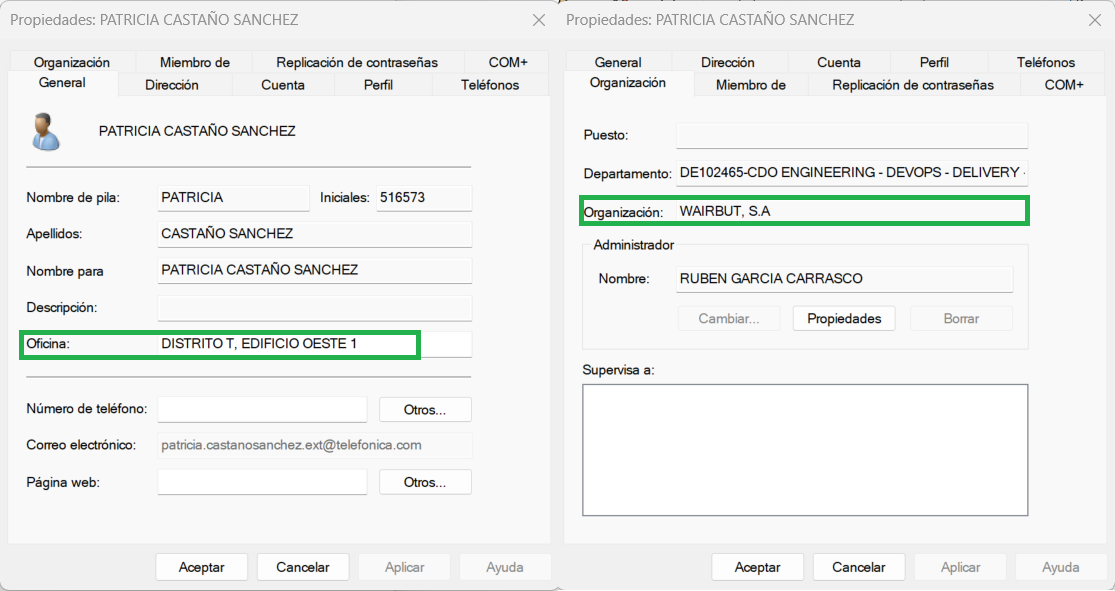
\includegraphics[width=15cm, height=8cm, keepaspectratio]{img/image01.png}
	\caption{Datos originales en Active Directory}
	\label{fig:image01}
\end{figure}

En la Figura 5.1 se ve la información que tiene el objeto del directorio activo antes de ejecutar el script de actualización de datos. Se requiere la atención en las propiedades del objeto ‘Organización’ y ‘Oficina’ ya que serán los datos que se actualizarán tras la ejecución del script.

\begin{figure}[h]
	\centering
	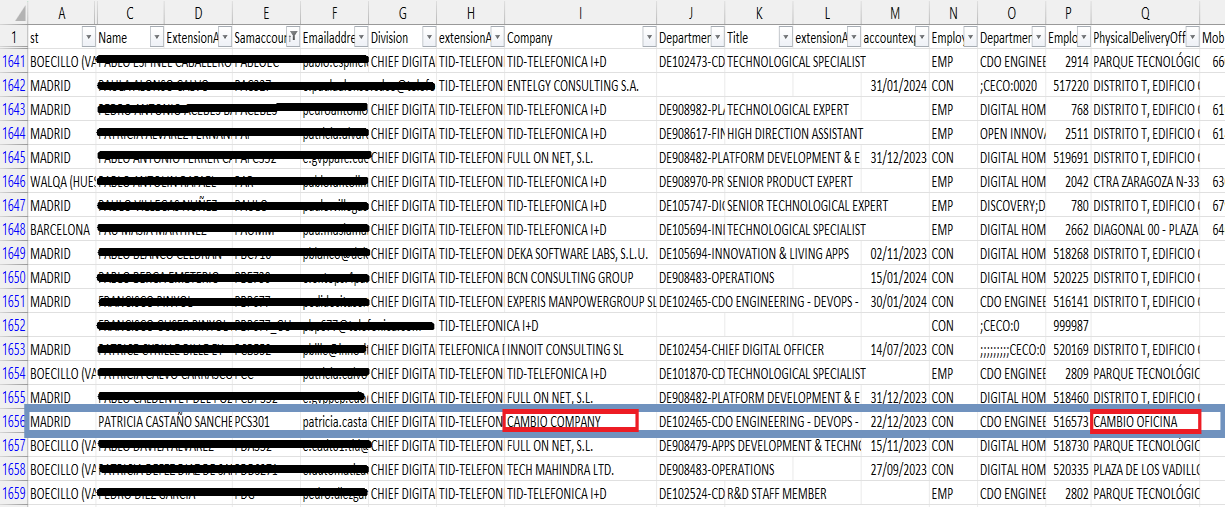
\includegraphics[width=15cm, height=8cm, keepaspectratio]{img/image02.png}
	\caption{Información en base de datos Oracle}
	\label{fig:image02}
\end{figure}

En la Figura 5.2 se ve la información que proviene de la base de datos Oracle, es la información ‘válida’ que debe contener el directorio activo. Se requiere especial atención en las columnas I y Q ya que, a propósito, se han modificado para mostrar el funcionamiento del script.

\begin{figure}[H]
	\centering
	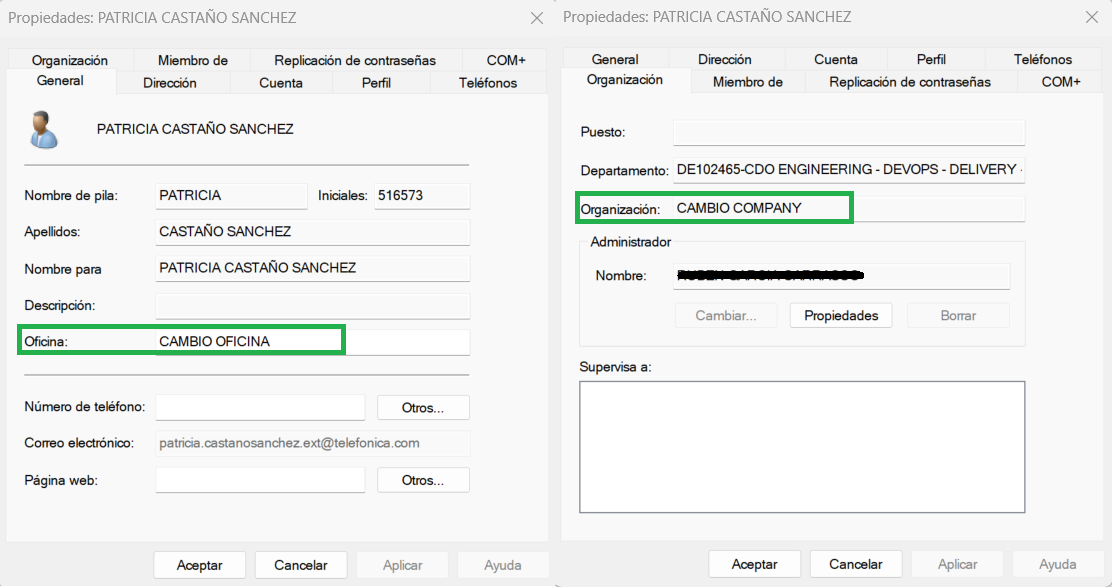
\includegraphics[width=15cm, height=8cm, keepaspectratio]{img/image03.png}
	\caption{Datos en Active Directory tras ejecutar el script}
	\label{fig:image03}
\end{figure}

En esta última figura se observa cómo, tras ejecutar el script de actualización de datos, las propiedades ‘Oficina’ y ‘Organización’ se han modificado.
\\

\item Experimento con colection-betaITuser-prepare.ps1

En este experimento se muestra cómo se generan dos colecciones de equipos en SCCM correspondientes a los usuarios almacenados en un grupo del directorio de Active Directory. El script se ejecuta en el servidor que tiene instalado el servicio de SCCM para evitar tener que ejecutarlo de manera remota desde otro servidor y hacer así más rápida su ejecución.

\begin{figure}[H]
	\centering
	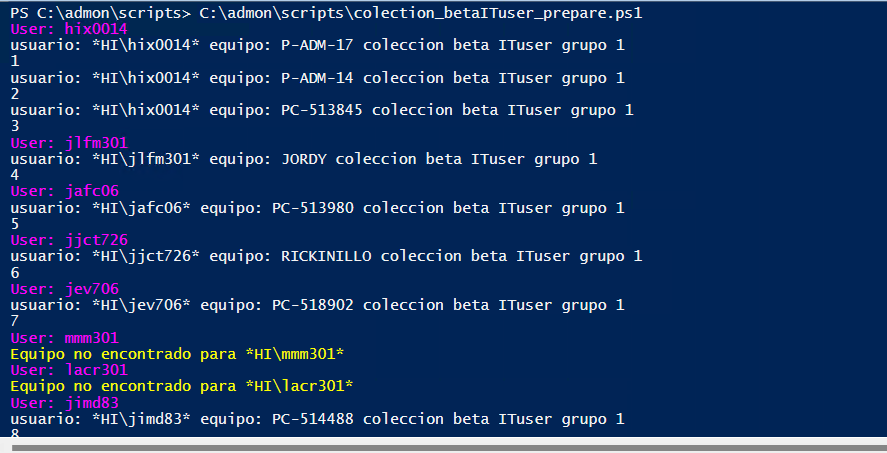
\includegraphics[width=15cm, height=8cm, keepaspectratio]{img/image04.png}
	\caption{Script en curso}
	\label{fig:image04}
\end{figure}

En la Figura 5.4 se muestra el script en curso que va sacando trazas durante su ejecución indicando a qué colección se está añadiendo cada equipo y un contador para ver cuántos equipos está añadiendo.

Se puede ver los equipos en SCCM que corresponden a cada usuario del grupo del directorio activo, así como si no encuentra ningún equipo para algún usuario.

\begin{figure}[H]
	\centering
	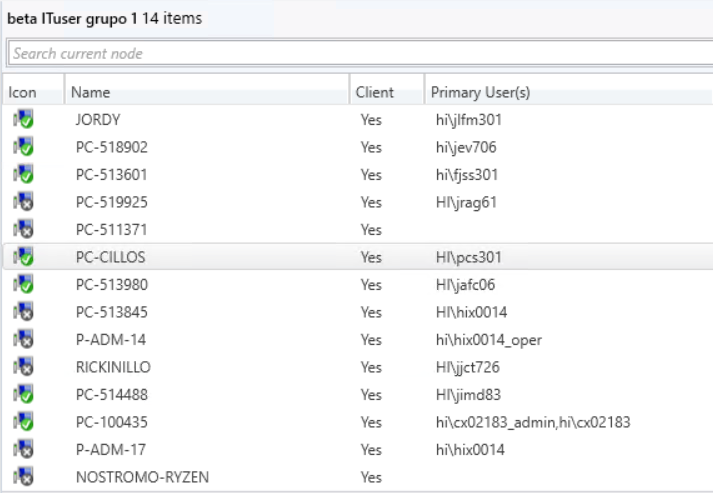
\includegraphics[width=15cm, height=8cm, keepaspectratio]{img/image05.png}
	\caption{Colección 1}
	\label{fig:image05}
\end{figure}


En la Figura 5.5 se muestra los equipos que ha añadido el script a la Colección 1 (beta ITUser grupo 1) en la herramienta de SCCM.
\\

\item Experimento con ExpiredPassword-ADUser.ps1

En este experimento se comprueba que, habiendo una contraseña que caducará en 15 días, el script, tras su ejecución, envía el aviso a la cuenta de correo asociada al usuario cuya contraseña va a caducar avisando de los días que le queda para cambiarla y de qué manera puede realizar este cambio.

\begin{figure}[H]
	\centering
	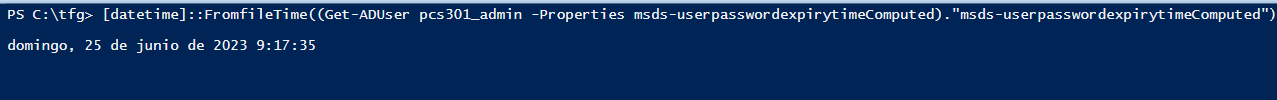
\includegraphics[width=15cm, height=8cm, keepaspectratio]{img/image06.png}
	\caption{Fecha de caducidad de contraseña en el AD}
	\label{fig:image06}
\end{figure}

En la Figura 5.6 se muestra la fecha en la que caduca la contraseña para el usuario utilizado en este experimento

\begin{figure}[H]
	\centering
	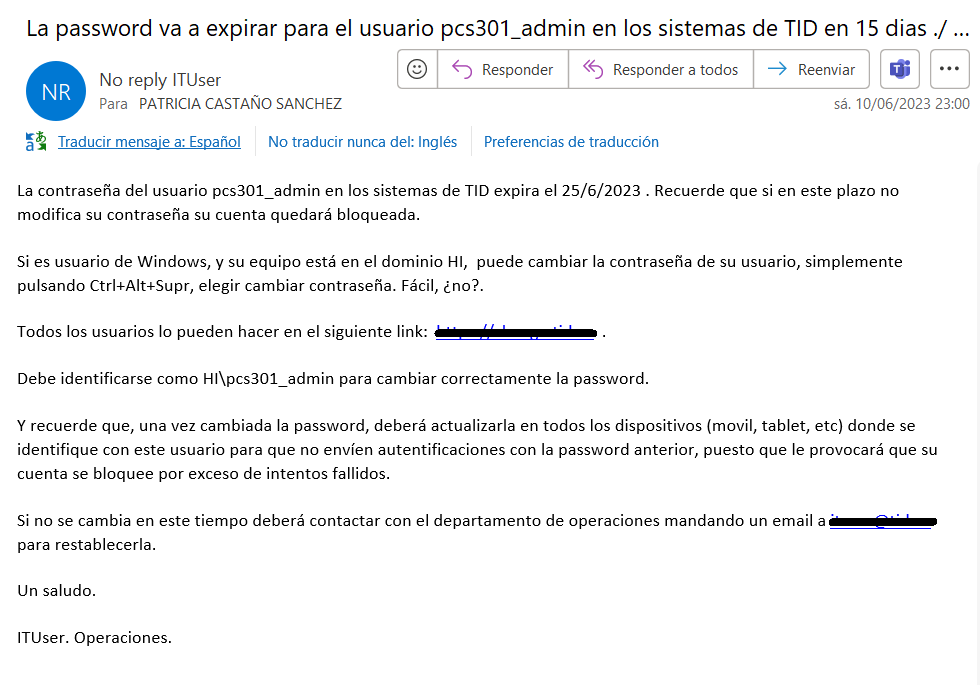
\includegraphics[width=15cm, height=8cm, keepaspectratio]{img/image07.png}
	\caption{Aviso de contraseña a punto de caducar}
	\label{fig:image07}
\end{figure}

En la Figura 5.7 se puede ver el correo electrónico que envía el script al usuario al que le va a caducar la contraseña.
\\

\item Experimento con Generate-UserCertificate.ps1

En este experimento se comprueba que, tras introducir el login del usuario del que se requiere certificado, el script conecta con el servidor que tiene el servicio de Central Administration, genera el certificado como se puede ver en la última imagen, y lo envía a la dirección de correo asociada al usuario del que se ha introducido el login, así como la contraseña para instalar dicho certificado.

\begin{figure}[H]
	\centering
	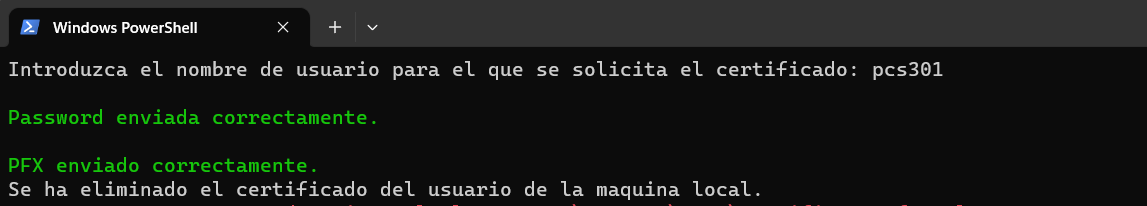
\includegraphics[width=15cm, height=8cm, keepaspectratio]{img/image08.png}
	\caption{Ejecución de script}
	\label{fig:image08}
\end{figure}

La Figura 5.8 muestra lo que aparece por pantalla cuando se ejecuta el script de generación de certificado, solicitando por pantalla el login del usuario al que se le quiere generar y enviar dicho certificado.

\begin{figure}[H]
	\centering
	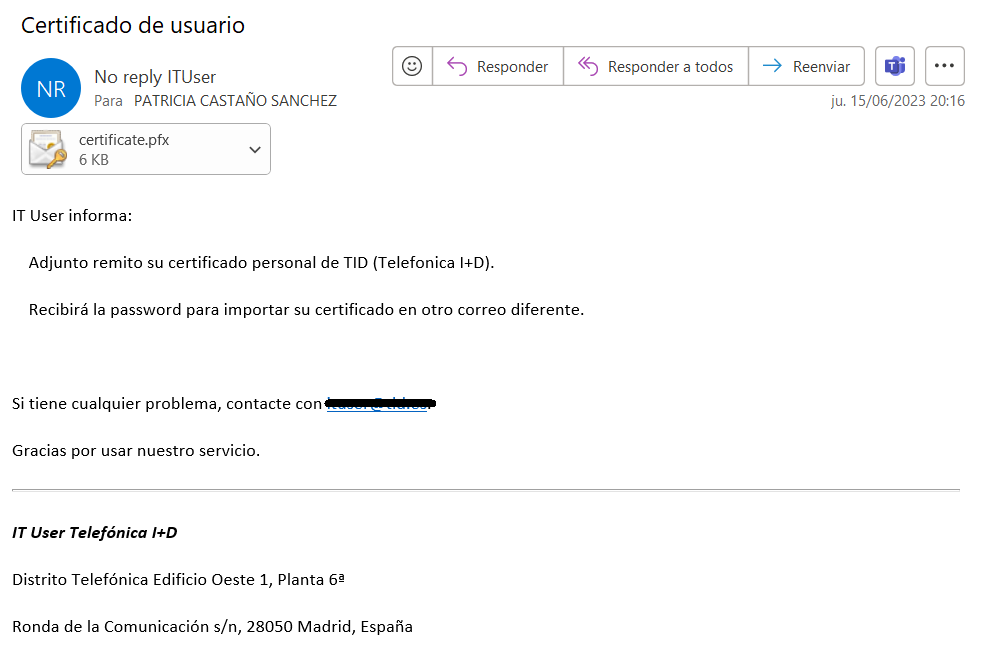
\includegraphics[width=15cm, height=8cm, keepaspectratio]{img/image09.png}
	\caption{Certificado enviado por correo}
	\label{fig:image09}
\end{figure}

\begin{figure}[H]
	\centering
	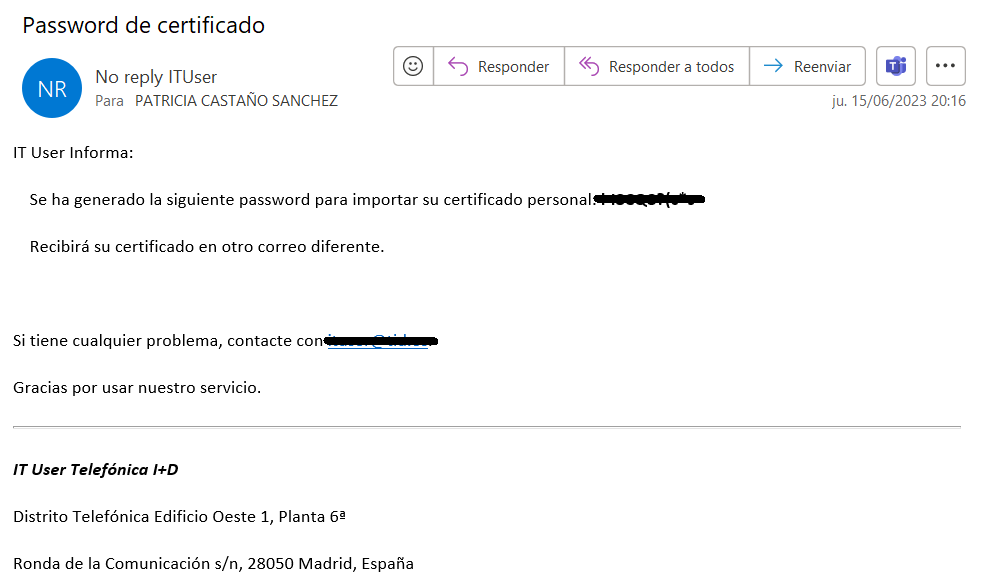
\includegraphics[width=15cm, height=8cm, keepaspectratio]{img/image10.png}
	\caption{Contraseña enviada por correo}
	\label{fig:image10}
\end{figure}

En la Figura 5.9 y la Figura 5.10 se puede ver los correos que envía el propio script adjuntando el certificado en uno de ellos, y la contraseña para instalar dicho certificado en otro. Esta información se envía en correos separados por si, en el hipotético caso de que se extraviaran los correos, cada correo por separa no se pudiera utilizar.

\begin{figure}[H]
	\centering
	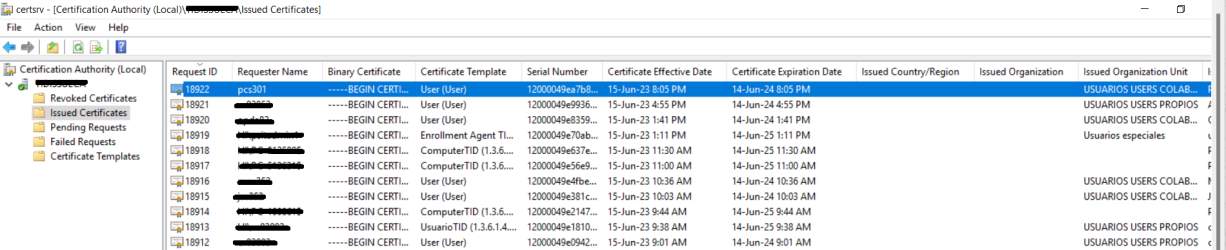
\includegraphics[width=15cm, height=8cm, keepaspectratio]{img/image11.png}
	\caption{Certificado en la CA}
	\label{fig:image11}
\end{figure}

En la Figura 5.11 aparece la Central Administration donde aparecen todos los certificados generados y se realza el certificado que acaba de generar el script.
\\

\item Experimento con Copy-SPItems.ps1

En este experimento se comprueba que, teniendo una lista de Sharepoint vacía, tras ejecutar el script, el cual nos solicita el nombre de la lista origen y la lista destino, se copian los datos de la lista destino en la lista origen.

\begin{figure}[H]
	\centering
	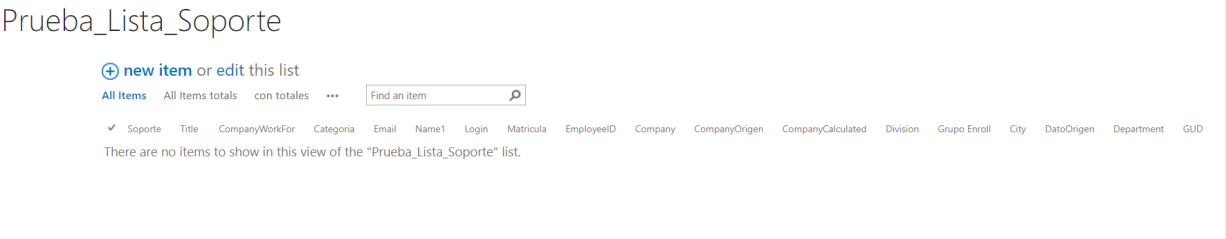
\includegraphics[width=15cm, height=8cm, keepaspectratio]{img/image12.png}
	\caption{Lista Sharepoint destino}
	\label{fig:image12}
\end{figure}

En la Figura 5.12 se muestra la lista destino, vacía antes de ejecutar el script.

\begin{figure}[H]
	\centering
	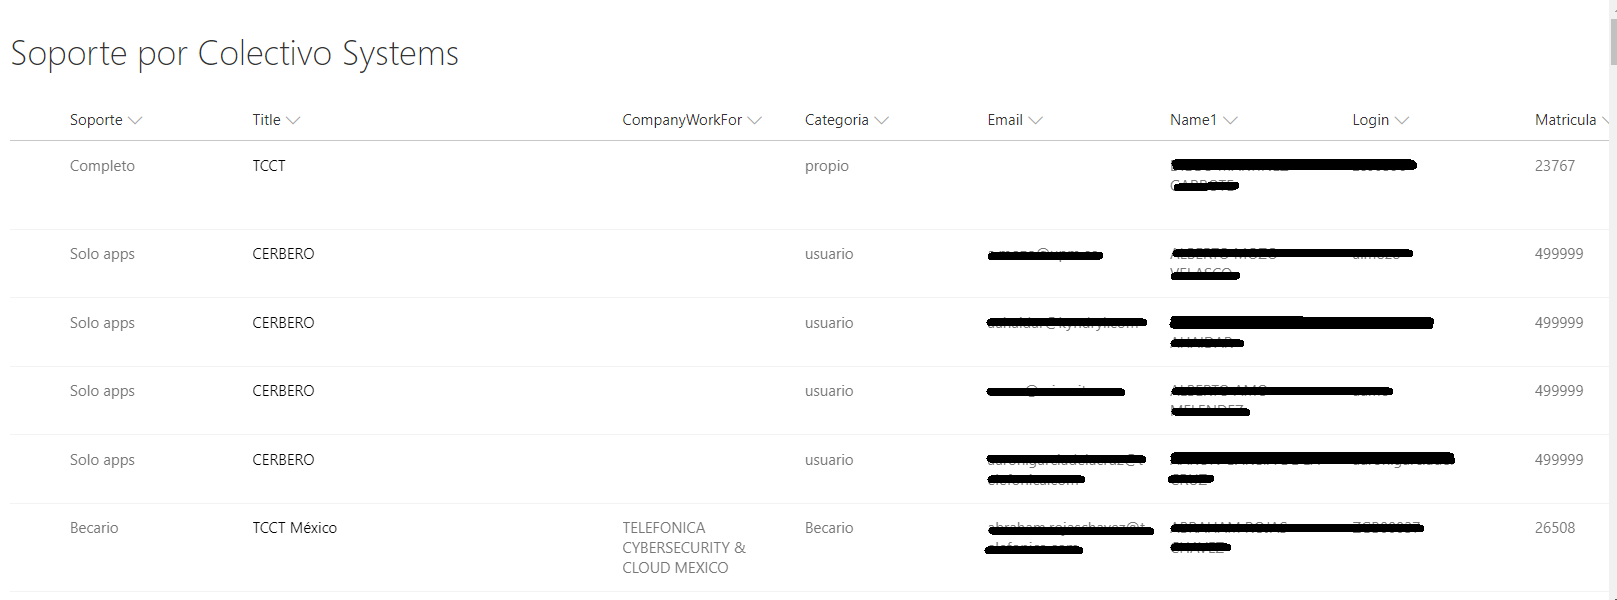
\includegraphics[width=15cm, height=8cm, keepaspectratio]{img/image13.png}
	\caption{Lista Sharepoint origen}
	\label{fig:image13}
\end{figure}

En la Figura 5.13 se muestra la lista origen, de la que se copiarán los ítems

\begin{figure}[H]
	\centering
	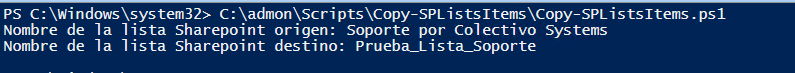
\includegraphics[width=15cm, height=8cm, keepaspectratio]{img/image14.png}
	\caption{Ejecución del script}
	\label{fig:image14}
\end{figure}

Cuando se ejecuta el script, se pide por pantalla el nombre de la lista de la que se copiarán los ítems, y el nombre de la lista donde se copiarán éstos.

\begin{figure}[H]
	\centering
	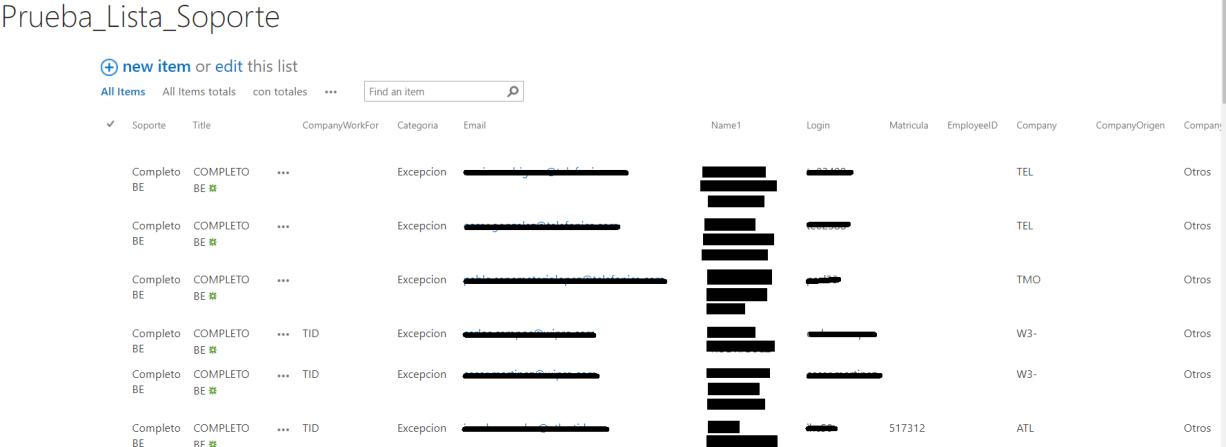
\includegraphics[width=15cm, height=8cm, keepaspectratio]{img/image15.png}
	\caption{Lista Sharepoint destino tras ejecutar el script}
	\label{fig:image15}
\end{figure}

En la Figura 5.15 vemos cómo se ha rellenado la lista que inicialmente estaba vacía.
\\

\item Experimento con Delete-SPItems.ps1

Con este experimento se comprueba que, teniendo una lista de Sharepoint llena, tras ejecutar el script en el que se le indica en el código el nombre de la lista que queremos vaciar, dicha lista queda limpia sin ningún ítem. Este script muestra por pantalla el número de ítems que contiene la lista y saca por pantalla una traza por cada ítem que va eliminando.

\begin{figure}[H]
	\centering
	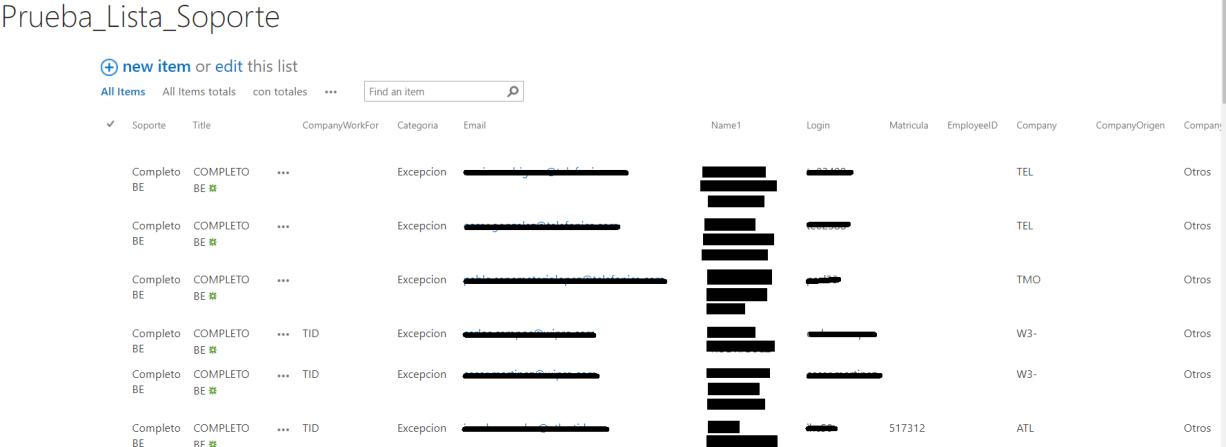
\includegraphics[width=15cm, height=8cm, keepaspectratio]{img/image15.png}
	\caption{Lista Sharepoint original rellena}
	\label{fig:image15}
\end{figure}

La Figura 5.16 muestra la lista original llena, antes de ejecutar el script de borrado.

\begin{figure}[H]
	\centering
	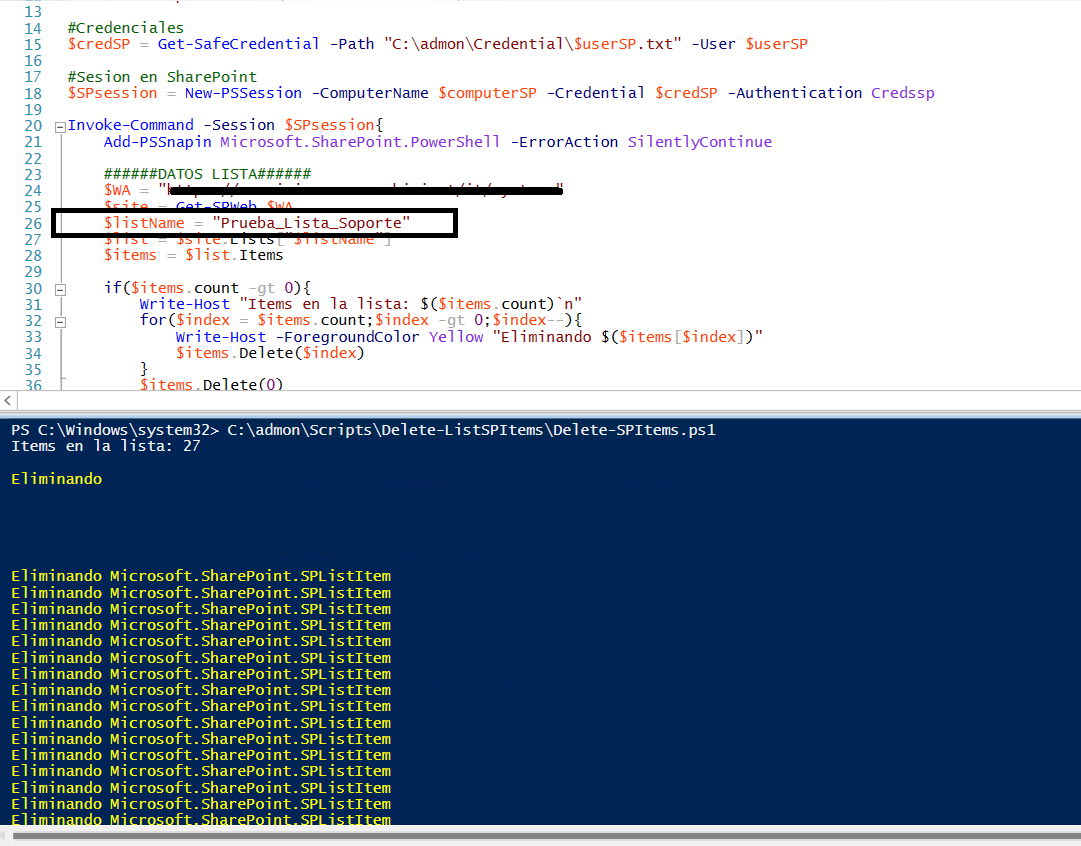
\includegraphics[width=15cm, height=8cm, keepaspectratio]{img/image16.png}
	\caption{Lista Sharepoint original rellena}
	\label{fig:image16}
\end{figure}

Es la Figura 5.17 se ve la ejecución del script, mostrando la línea de código donde se modifica el nombre de la lista que se quiere vaciar (línea 26 del script). En la consola de Powershell vemos una traza por cada ítem eliminado para ir comprobando que el script se está ejecutando correctamente.

\begin{figure}[H]
	\centering
	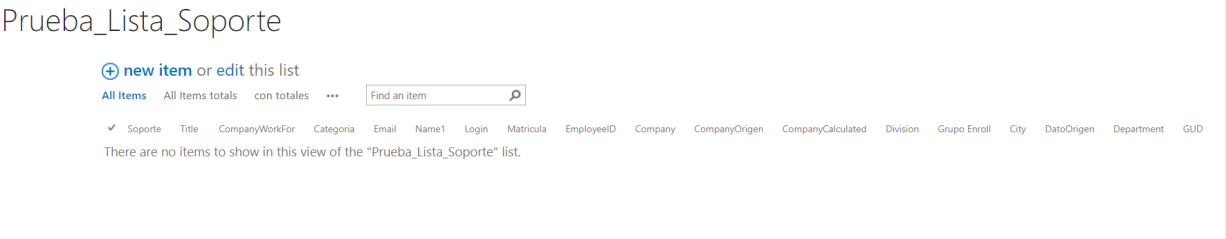
\includegraphics[width=15cm, height=8cm, keepaspectratio]{img/image12.png}
	\caption{Lista Sharepoint vaciada}
	\label{fig:image12}
\end{figure}

La Figura 5.18 muestra la lista tras ejecutar el script. Se puede comprobar que se han eliminado los ítems de ella.

\end{itemize}


%%%%%%%%%%%%%%%%%%%%%%%%%%%%%%%%%%%%%%%%%%%%%%%%%%%%%%%%%%%%%%%%%%%%%%%%%%%%%%%%
%%%%%%%%%%%%%%%%%%%%%%%%%%%%%%%%%%%%%%%%%%%%%%%%%%%%%%%%%%%%%%%%%%%%%%%%%%%%%%%%
% CONCLUSIONES %
%%%%%%%%%%%%%%%%%%%%%%%%%%%%%%%%%%%%%%%%%%%%%%%%%%%%%%%%%%%%%%%%%%%%%%%%%%%%%%%%

\cleardoublepage
\chapter{Conclusiones}
\label{chap:conclusiones}


\section{Consecución de objetivos}
\label{sec:consecucion-objetivos}

El objetivo en este proyecto era demostrar que se puede simplificar y facilitar el trabajo del técnico en una empresa de IT automatizando tareas repetitivas y densas. Tras mostrar varios ejemplos de tareas automatizadas, se demuestra que es posible simplificar y facilitar una tarea larga y repetitiva ejecutando un script, o incluso transformando un script en una tarea automática.
\\

Antes de la automatización de tareas, los trabajadores ejecutaban de forma manual y a diario muchas de las tareas mostradas en este trabajo, lo que les llevaba muchas horas realizar una tarea que, gracias a los scripts, se ha reducido a minutos. Pudiendo, además, desatender la tarea mientras se está ejecutando el script y poder dedicarse a otras labores de la empresa.


\section{Aplicación de lo aprendido}
\label{sec:aplicacion}

En varias asignaturas del Grado se enseña lenguajes de programación, esto ayuda a desarrollar la capacidad de resolver un mismo problema con diferentes puntos de vista y con diferentes métodos de actuación. Esto me ha ayudado en mi empresa a que, cuando se presenta una problemática, o una nueva tarea para automatizar, ser rápida a la hora de encontrar posible soluciones y formas de llevarlas a cabo.
\\

El trabajo fin de grado está basado en el lenguaje de scripting Powershell, un lenguaje que no aprendí en el Grado pero que, gracias al desarrollo que tuve con diferentes lenguajes en la Universidad, fui capaz de aprenderlo en un corto plazo de tiempo.

%%%%%%%%%%%%%%%%%%%%%%%%%%%%%%%%%%%%%%%%%%%%%%%%%%%%%%%%%%%%%%%%%%%%%%%%%%%%%%%%
%%%%%%%%%%%%%%%%%%%%%%%%%%%%%%%%%%%%%%%%%%%%%%%%%%%%%%%%%%%%%%%%%%%%%%%%%%%%%%%%
% REFERENCIAS %
%%%%%%%%%%%%%%%%%%%%%%%%%%%%%%%%%%%%%%%%%%%%%%%%%%%%%%%%%%%%%%%%%%%%%%%%%%%%%%%%

\cleardoublepage
\chapter{Referencias}
\label{chap:Referencias}

\url{https://www.microsoft.com}
\\

\url{https://www.learn.microsoft.com}
\\

\url{https://learn.microsoft.com/es-es/powershell/scripting/overview?view=powershell-7.3}
\\

\url{https://support.microsoft.com/es-es/office}
\\

\url{https://www.oracle.com}
\\

\url{https://www.google.es}


\end{document}
